\documentclass[oneside,a4paper,11pt,explicit]{book}
\usepackage[utf8]{inputenc}
\usepackage{icecream}
\usepackage[english]{babel}
\addto\captionsenglish{\renewcommand{\chaptername}{}}
\usepackage[accsupp]{axessibility}  % improves PDF readability for those with disabilities.
\usepackage[colorlinks = true,urlcolor  = blue,linkcolor = blue]{hyperref}
\usepackage{setspace}
\usepackage{listings}
\usepackage[most]{tcolorbox}
\usepackage{minitoc}
\usepackage{multicol}


\renewcommand{\mtifont}{\large\sffamily}
\renewcommand{\mtcfont}{\small\sffamily}
\renewcommand{\mtcSfont}{\small\sffamily}
\renewcommand{\mtcSSfont}{\small\sffamily}
\renewcommand{\mtcSSSfont}{\small\sffamily}
\mtcsetpagenumbers{minitoc}{off} % turn off page numbering in minitocs
\addto{\captionsenglish}{% Making babel aware of special titles
	\renewcommand{\mtctitle}{Quick Links To Sections}
}
\setlength{\fboxrule}{5pt}
\setlength{\fboxsep}{4pt}

\definecolor{IceCreamLeaf}{rgb}{0.4, 0.639215686274, 0.4}
\definecolor{IceCreamOrbit}{rgb}{0.803921568627451, 0.3607843137254902, 0.3607843137254902}

\title{I.C.E.C.R.E.A.M. Tutorials}
\subtitle{\small Observing Earth from Above (Env 329) - Fall 2023  \\
	\small Schmid College of Science and Technology, Chapman University}
\date{\today}

%% DOCUMENT
\setstretch{1.25}
\makeatletter
\begin{document}

\setcounter{tocdepth}{3}
\setcounter{minitocdepth}{3}
\dominitoc
%\tableofcontents

\setcounter{chapter}{8} %Insert (Tutorial Number-1) Here; example for tutorial 4, enter 3

\chapter{Communicating Data} %Enter Tutorial Name Here

\vspace{-2em}

\minitoc

\hrule

\vspace{1em}

\begin{tcolorbox}[enhanced,frame style image=blueshade.png,
	opacityback=0.75,opacitybacktitle=0.25,
	colback=blue!5!white,colframe=blue!75!black,title={\Large \textbf{Objectives:}}]
	\large
	\begin{enumerate}
		\item Learn how to access colorbrewer options in QGIS.
		\item Incorporate Dr. Davidoff's data communication ideas into our ECOSTRESS workflow.
	\end{enumerate}
\end{tcolorbox}

\clearpage

%%%%%%%%%%%%%%%%%%%%%%%%%%%%%%%%%% Change Header to Have a Smaller Logo for Remainder of the Document
\fancyhead{}
\fancyhead[C]{\begin{tikzpicture}[overlay, remember picture]
		\fill[Blue2] (current page.north west) rectangle ($(current page.north east)+(0,-1in)$);
		\node[anchor=north west, text=white, font=\Large, minimum size=1in, inner xsep=5mm, align=left] at (current page.north west) {\bf{\MakeUppercase{\@title}}\\\@subtitle};
		\node[anchor=north east, minimum size=1in, inner xsep=5mm] at (current page.north east) {\includegraphics[scale=.125]{ICECREAM_Logo.png}};\end{tikzpicture}}
%%%%%%%%%%%%%%%%%%%%%%%%%%%%%%%%%%

\noindent\fbox{\begin{minipage}{.9665\textwidth}
			
	\vspace{1em}
	\begin{center}
		\textbf{\Large \underline{Motivation For Today's Tutorial : Communicating Science}}
	\end{center}
	
	\addcontentsline{toc}{section}{Motivation : Communicating Science}

	\vspace*{-1 em}
	
	\centerline{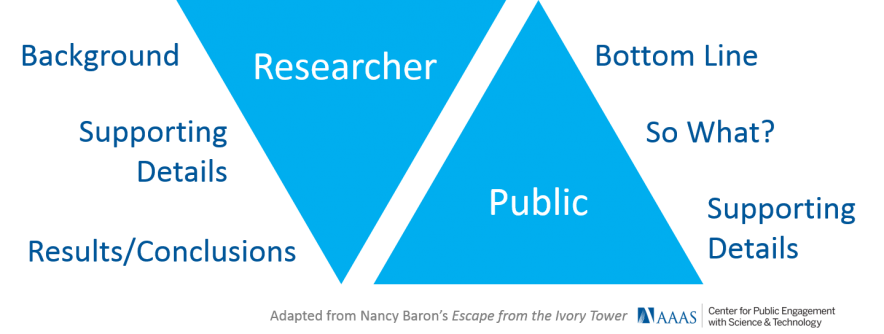
\includegraphics[width=.87\textwidth]{AAAS_CommunicationTriangle.png}}

	The following is an excerpt from the National Institute of Health's Article ``Communicating Science Effectively: A Research Agenda.'':

	\vspace{.5em}

	\textit{The public generally holds scientists and their work in high regard due to the contributions science has made to the daily lives of those in society, and science in turn has benefited from substantial financial and other forms of public support. This mutually supportive relationship between science and society places a responsibility on scientists and technologists, as citizens, to share the results of their work with the broader public so they can reap its benefits as expeditiously as possible.}

	\vspace{.5em}

	\textit{Communicating about science effectively with public audiences, however, turns out to be more difficult than it might appear at first. Complexity stems from the diversity and interconnectedness of many elements, including the goals for communicating, the content being conveyed, the format in which it is presented, and the individuals and organizations involved. People approach science communication from their own starting points; a combination of expectations, knowledge, skills, beliefs, and values that are in turn shaped by broader social, political, and economic influences.}

	\vspace{.5em}

	\textit{Moreover, the communication landscape is changing dramatically in ways that offer unprecedented opportunities to communicate and connect with others, but also pose many challenges.}

	\vspace{.5em}

	In the last class, Dr. Davidoff presented some new ideas on communicating data. Today, we are going to incorporate those ideas into our ECOSTRESS workflow.
	
\end{minipage}}

\section{Using ColorBrewer In QGIS}

Dr. Davidoff introduced ColorBrewer for selecting preset color palettes to make visualizing our data easier. While you can manually edit color ramps in QGIS, many of the ColorBrewer palettes are already available in QGIS through the \textit{Style Manager}. 

1. To access the style manager, open QGIS and select \textit{Settings}, then \textit{Style Manager}.

2. Select \textit{Color Ramps}

3. Use the ``+'' sign to select \textit{Catalog: ColorBrewer}.

\centerline{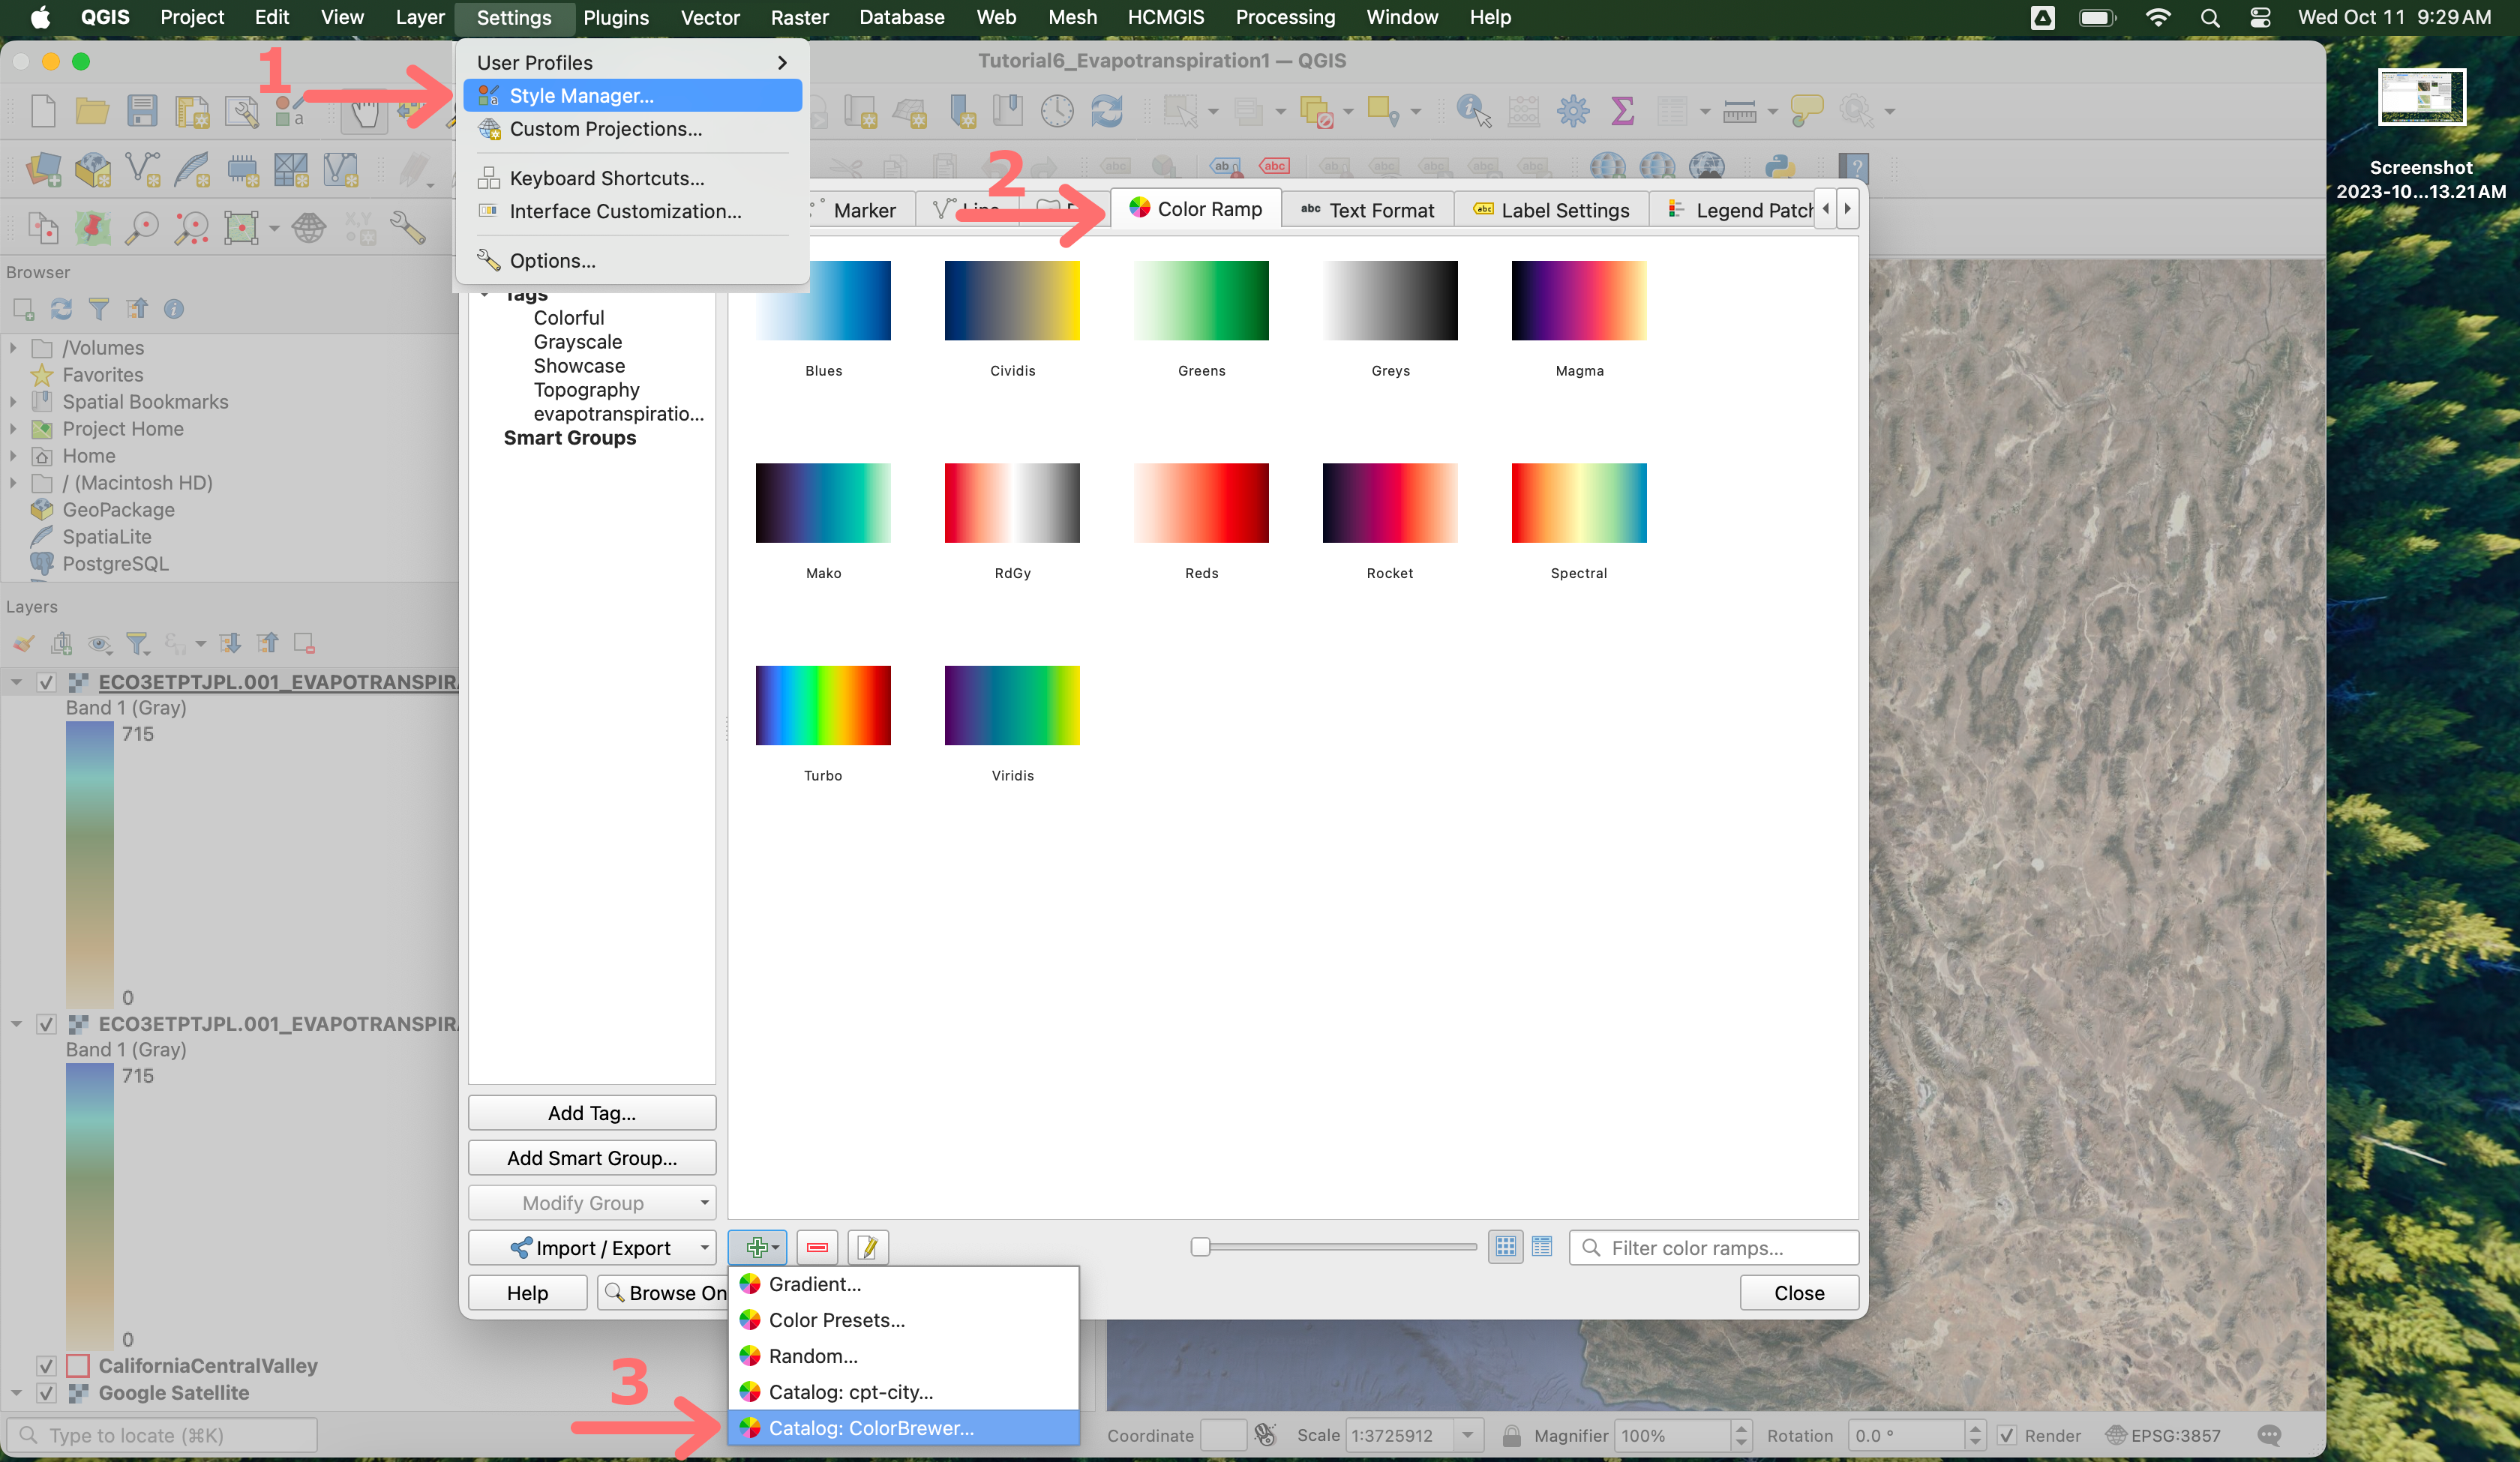
\includegraphics[width=.87\textwidth]{StyleManager.png}}

\vspace{.5em}

\centerline{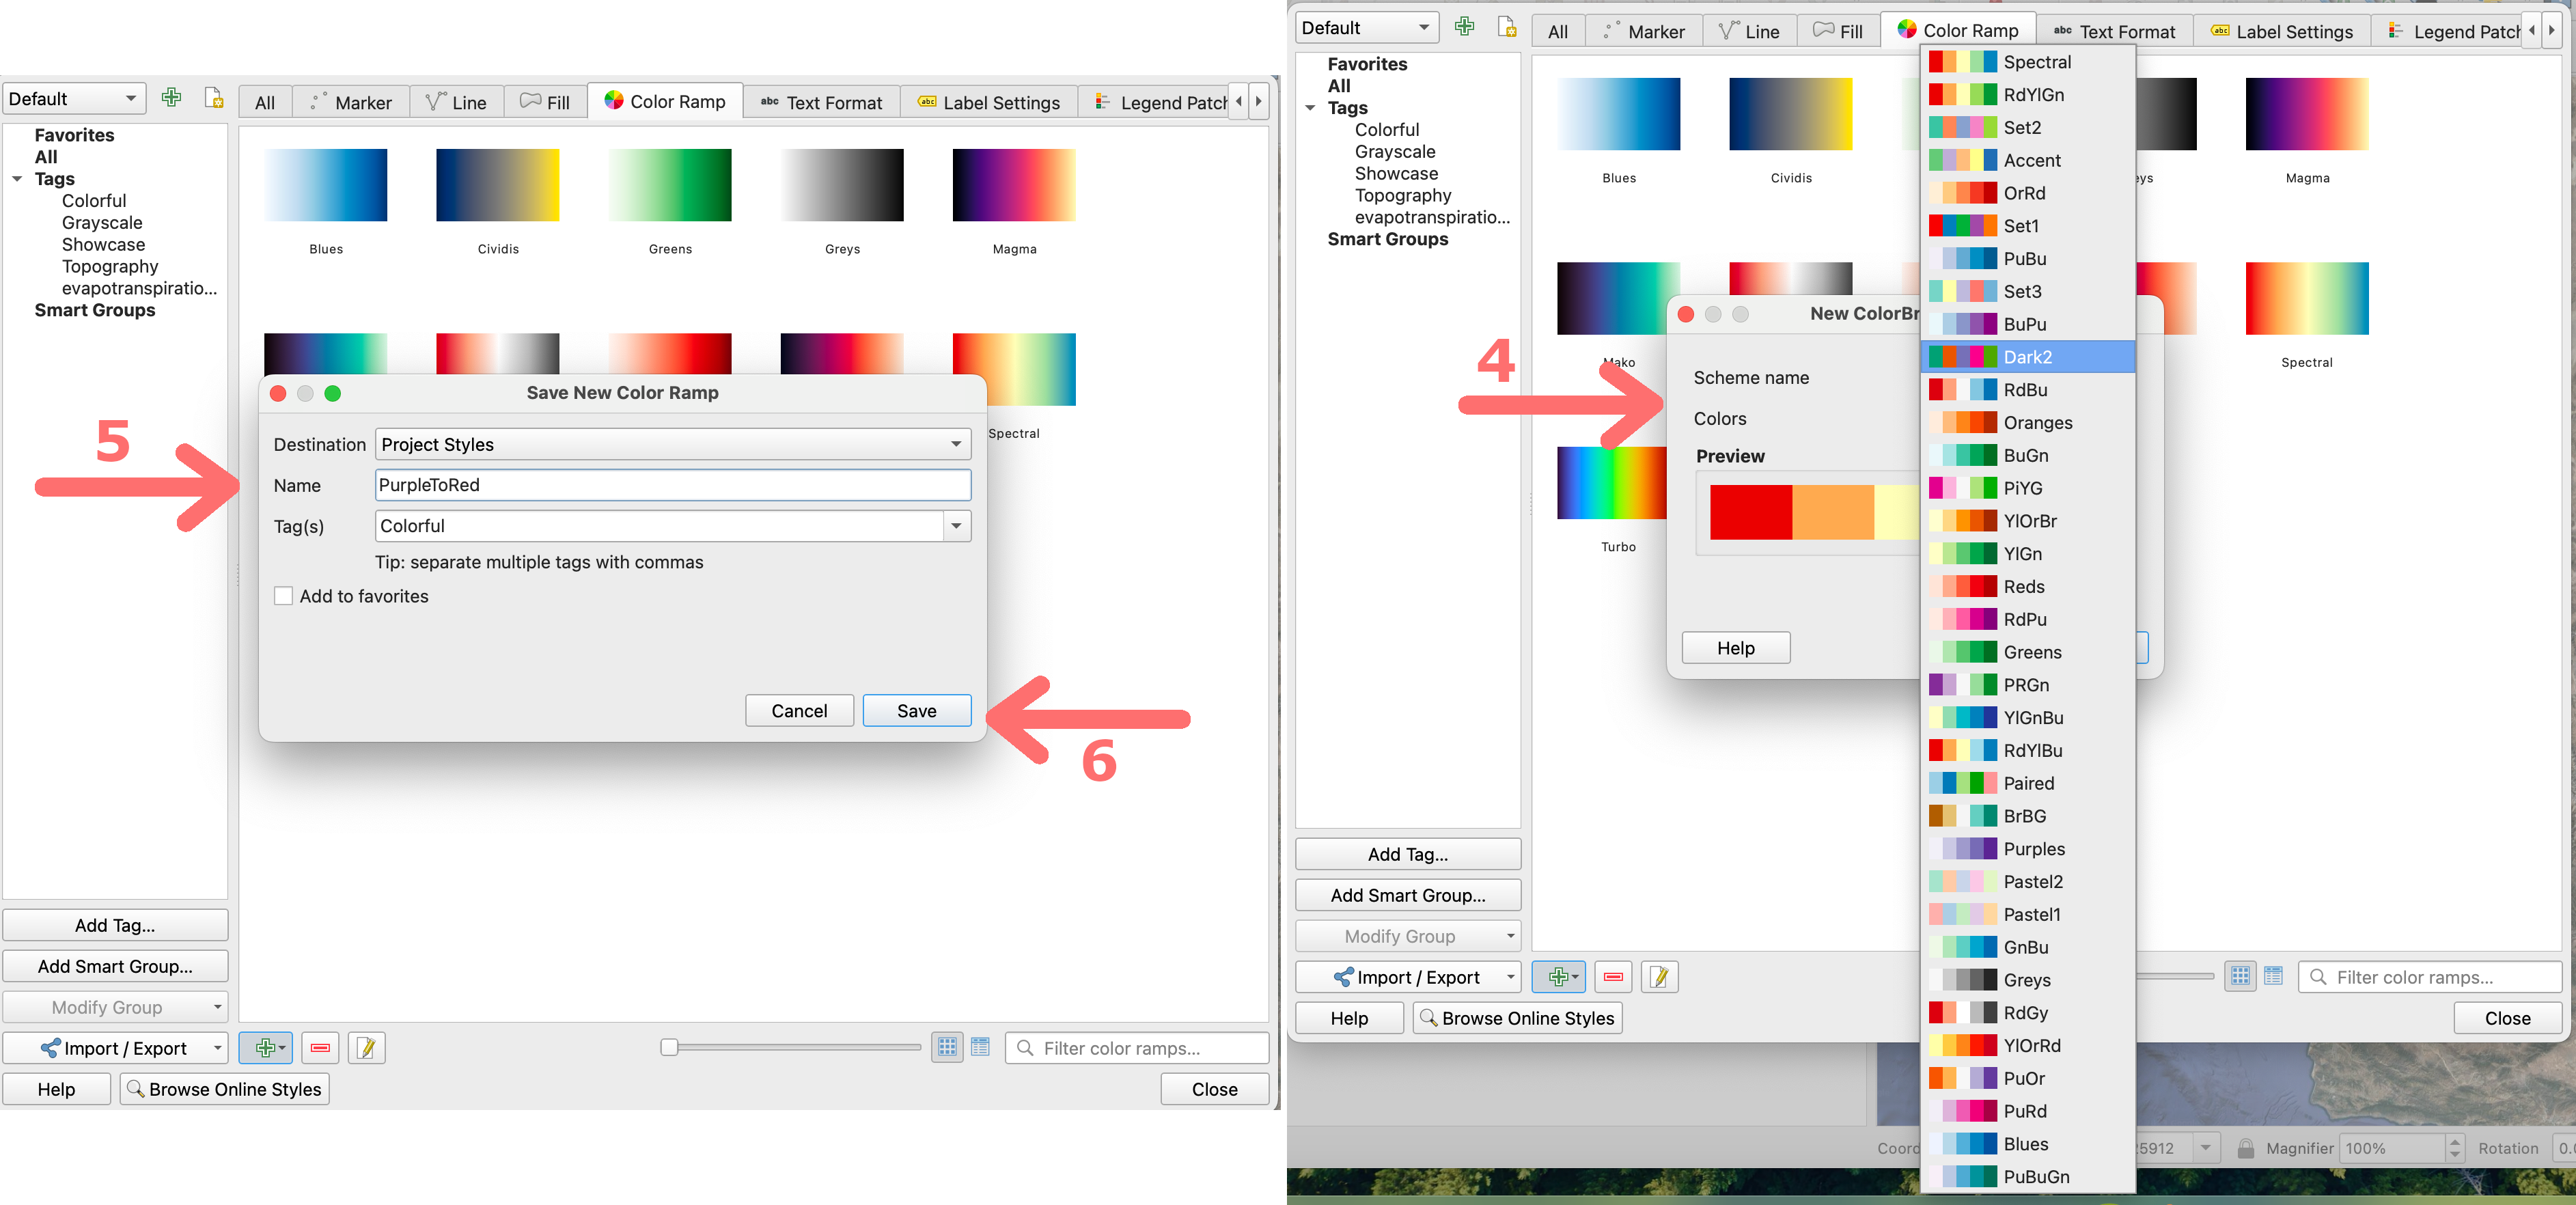
\includegraphics[width=.87\textwidth]{QGIScolorBrewer.png}}

\vspace{.5em}

4. From this screen, you can select from preset color schemes and the number of color classes you want.

5. After you click \textit{OK}, QGIS prompts you to name and save your new color ramp. Pick a name that you can remember. If you think that you will use this color ramp often, you can click the ``Add to favorites'' box. 

6. Click \textit{Save}.

7. This color ramp can now be accessed by right clicking on a layer, selecting the \textit{Symbology} tab, then the little down arrow next to the color ramp bar. Under the heading ``All Color Ramps'' you should find your new ramp. See the screenshot below for where to look. NOTE: If you have marked it as a favorite, it shows up in the first list. 

\centerline{\includegraphics[width=.87\textwidth]{UseColorRamp.png}}

\vspace{.5em}

\section{Instructions From Dr. Davidoff}

For the remainder of today's class, we are going to work through an assignment created by Dr. Davidoff.

\begin{enumerate}
    \item Redesign a previous map, using the principles of graphical communication:
	\begin{itemize}
		\item What are the variables your map displays, and what visual dimensions are you using to encode that data? What color palette are you using and why?
		\item How are you following the principle of data/ink ratio? Do you have any unnecessary lines? Can your line strokes be reduced in weight? What are you using as your base map and why?
		\item What \href{https://en.wikipedia.org/wiki/Map_layout}{map layout }are you using? Are the panels the same size? Similarly justified? Do they have titles and captions that explain their contents? Is there a hierarchy of size in the type?
		\item Are you following the principles of gestalt psychology? Are related items physically proximal? Are unrelated items standalone?
        \end{itemize}
    \item Once you have redesigned your map, trade with one of your classmates and discuss the choices you made in your redesign. Is there anything you wish to further revise? 
    \item Find an environmental event (e.g., climate disaster) that occurred in the past week. Download relevant ECOSTRESS data (LST, ET, WUE, ESI) for that location. Make a map using best practices for data visualization. Write a 4-6 sentence paragraph (topic sentence, supporting description, relevant conclusion) describing the event to accompany the map.
\end{enumerate}

\begin{tcolorbox}[colback=yellow!5!white,colframe=IceCreamOrbit,title= \vspace{.2em} \Large Map of the Week Assignments]
	\addcontentsline{toc}{section}{Map of the Week Assignments}
	\large
	\begin{enumerate}
		\item Submit your redesigned map following the instructions above. 
		\item Submit your environmental event map following the above instructions. 
	\end{enumerate}
	Submit these assignments via Canvas before the next class.
\end{tcolorbox}

%%%%%%%%%%%%%%%%%%%%%%%%%%%%%%%%%%%%%%%%%%%%%%%%%%%%%%%%%%%%%%%%%%%%%%%%%%%%%%%%%%% End of Document
%\vfill

\hrule

\vspace{1em}

\small \textbf{Recommended Citation:} Forsythe, J.D., G.R. Goldsmith, and J.B. Fisher. 2023. Observing Earth from Above Tutorials. Chapman University. \url{https://jeremydforsythe.github.io/icecream-tutorials/}

\vspace{1em}

This work is supported by funding from NASA ECOSTRESS Mission Grant \#80NSSC23K0309 (I.C.E. C.R.E.A.M.: Integrating Communication of ECOSTRESS Into Community Research, Education, Applications, and Media).

\end{document}
